% Template file for an a0 landscape poster.
% Written by Graeme, 2001-03 based on Norman's original microlensing
% poster.
%
% See discussion and documentation at
% <http://www.astro.gla.ac.uk/users/norman/docs/posters/> 
%
% $Id: poster-template-landscape.tex,v 1.2 2002/12/03 11:25:46 norman Exp $
	

% Default mode is landscape, which is what we want, however dvips and
% a0poster do not quite do the right thing, so we end up with text in
% landscape style (wide and short) down a portrait page (narrow and
% long). Printing this onto the a0 printer chops the right hand edge.
% However, 'psnup' can save the day, reorienting the text so that the
% poster prints lengthways down an a0 portrait bounding box.
%
% 'psnup -w85cm -h119cm -f poster_from_dvips.ps poster_in_landscape.ps'

\documentclass[a0]{a0poster}


% You might find the 'draft' option to a0 poster useful if you have
% lots of graphics, because they can take some time to process and
% display. (\documentclass[a0,draft]{a0poster})
\input defs
\pagestyle{empty}
\setcounter{secnumdepth}{0}
\renewcommand{\familydefault}{\sfdefault}
\newcommand{\QED}{~~\rule[-1pt]{8pt}{8pt}}\def\qed{\QED}

\renewcommand{\reals}{{\mbox{\bf R}}}

% The textpos package is necessary to position textblocks at arbitary 
% places on the page.
\usepackage[absolute]{textpos}

\usepackage{fleqn,psfrag,wrapfig,tikz}

\usepackage[papersize={38in,28in}]{geometry}
\usepackage{array,tabularx,tabulary,booktabs} % Дополнительная работа с таблицами
\usepackage{longtable}  % Длинные таблицы
\usepackage{multirow} % Слияние строк в таблице
\usepackage{graphicx}
\usepackage{fancyhdr}
\usepackage{hyperref}
\usepackage{booktabs}
\usepackage{ upgreek }
\usepackage{euscript}	 % Шрифт Евклид
\usepackage{mathrsfs} % Красивый матшрифт
\usepackage{graphicx,array}

%\usepackage{extsizes} % Возможность сделать 14-й шрифт
\usepackage{geometry} % Простой способ задавать поля

\usepackage{chngcntr}
\usepackage{hyperref}
\usepackage{amsfonts,amssymb,amsthm,mathtools} % AMS
\usepackage{amsmath}
\usepackage{icomma}
\usepackage{multirow}

% Graphics to include graphics. Times is nice on posters, but you
% might want to switch it off and go for CMR fonts.
\usepackage{graphics}


% we are running pdflatex, so convert .eps files to .pdf
%\usepackage[pdftex]{graphicx}
%\usepackage{epstopdf}

% These colours are tried and tested for titles and headers. Don't
% over use color!
\usepackage{color}
\definecolor{Red}{rgb}{0.9,0.0,0.1}

\definecolor{bluegray}{rgb}{0.15,0.20,0.40}
\definecolor{bluegraylight}{rgb}{0.35,0.40,0.60}
\definecolor{gray}{rgb}{0.3,0.3,0.3}
\definecolor{lightgray}{rgb}{0.7,0.7,0.7}
\definecolor{darkblue}{rgb}{0.2,0.2,1.0}
\definecolor{darkgreen}{rgb}{0.0,0.5,0.3}

\renewcommand{\labelitemi}{\textcolor{bluegray}\textbullet}
\renewcommand{\labelitemii}{\textcolor{bluegray}{--}}

\setlength{\labelsep}{0.5em}

\newcommand{\lt}{\left}
\newcommand{\rt}{\right}
\newcommand{\al}{\alpha}
\newcommand{\p}{\partial}
\newcommand{\D}{\Delta}
\newcommand{\fr}{\frac}
\newcommand{\dfr}{\dfrac}
\newcommand{\mbf}{\mathbf}
\newcommand{\bb}{\mathbb}
\newcommand{\wt}{\widetilde}
\newcommand{\La}{\Lambda}
\newcommand{\la}{\lambda}
\newcommand{\opn}{\operatorname}

% see documentation for a0poster class for the size options here
\let\Textsize\normalsize
%\def\Head#1{\noindent\hbox to \hsize{\hfil{\LARGE\color{bluegray} #1}}\bigskip}
\def\Head#1{\noindent{\LARGE\color{bluegray} #1}\bigskip}
\def\LHead#1{\noindent{\LARGE\color{bluegray} #1}\bigskip}
\def\Subhead#1{\noindent{\large\color{bluegray} #1}\bigskip}
\def\Title#1{\noindent{\VeryHuge\color{Red} #1}}


% Set up the grid
%
% Note that [40mm,40mm] is the margin round the edge of the page --
% it is _not_ the grid size. That is always defined as 
% PAGE_WIDTH/HGRID and PAGE_HEIGHT/VGRID. In this case we use
% 23 x 12. This gives us three columns of width 7 boxes, with a gap of
% width 1 in between them. 12 vertical boxes is a good number to work
% with.
%
% Note however that texblocks can be positioned fractionally as well,
% so really any convenient grid size can be used.
%
\TPGrid[30mm,15mm]{23}{12}      % 3 cols of width 7, plus 2 gaps width 1

\parindent=0pt
\parskip=0.1\baselineskip


\begin{document}

% Understanding textblocks is the key to being able to do a poster in
% LaTeX. In
%
%    \begin{textblock}{wid}(x,y)
%    ...
%    \end{textblock}
%
% the first argument gives the block width in units of the grid
% cells specified above in \TPGrid; the second gives the (x,y)
% position on the grid, with the y axis pointing down.

% You will have to do a lot of previewing to get everything in the 
% right place.

% This gives good title positioning for a portrait poster.
% Watch out for hyphenation in titles - LaTeX will do it
% but it looks awful.
\begin{textblock}{23}(0,0)
\Title{Benchmarking of quasi-Newton methods}
\end{textblock}

\begin{textblock}{23}(0,0.6)
{
\LARGE
Igor Sokolov
}

{
\Large
\color{bluegray}
\emph{Optimization Class Project. MIPT}
}
\end{textblock}
% Uni logo in the top right corner. A&A in the bottom left. Gives a
% good visual balance, but you may want to change this depending upon
% the graphics that are in your poster.
%\begin{textblock}{2}(0,10)
%Your logo here
%%\includegraphics{/usr/local/share/images/AandA.epsf}
%\end{textblock}

%\begin{textblock}{2}(21.2,0)
%Another logo here
%%\resizebox{2\TPHorizModule}{!}{\includegraphics{/usr/local/share/images/GUVIu/GUVIu.eps}}
%\end{textblock}
\begin{textblock}{7.1}(0,1.5)
	
\hrule\medskip
\Head{Introduction}\\
The most well-known minimization technique for unconstrained problems is Newton’s Method.
In each iteration, the step update is $x_{k+1} = x_k - \lt(\nabla^2f_k\rt)\nabla f_k$.
Ноwever, the inverse of the Hessian has to be calculated in every
iteration so it takes $O\lt(n^3\rt)$. Moreover, in some applications, the second derivatives
may be unavailable. One fix to the problem is to use a finite difference approximation to
the Hessian.

We consider solving the nonlinear unconstrained minimization problem
$$\min f(x), x \in \bb{R}$$
Let's consider the following quadratic model of the objective function

$m_k(p) = f_k + \nabla f_k^Tp + \fr{1}{2}B_kp$, 
where $B_k = B_k^T, B_k \succ 0$ is an $n \times n$

The minimizer $p_k$ of this convex quadratic model
$p_k =  - B_k^{-1}\nabla f_k$
is used as the search direction, and the new iterate is 

$x_{k+1} = xk + \al p_k$, let $s_k = \al p_k$


The general structure of quasi-Newton method can be summarized as follows

\begin{itemize}
\item Given $x_0$, $B_0$(or $H_0$), $k \rightarrow 0;$

\item \textbf{For} $k = 0, 1, 2, \dots$

\quad Evaluate gradient $g_k$.

\quad Calculate $s_k$ by line search or trust region methods.

\quad $x_{k+1} \leftarrow x_k + s_k$

\quad $y_k \leftarrow  g_{k+1} - g_k$

\quad Update $B_{k+1}$ or $H_{k+1}$ according to the quasi-Newton formulas.

\textbf{End(for)}

\end{itemize}
Basic requirement in each iteration, i.e.,
$B_k s_k = y_k$ (or $H_k y_k = s_k$)

\hrule\medskip
\Head{ Quasi-Newton Formulas for Optimization}
\begin{flushleft}
	\begin{tabular}{ p{10cm} p{16cm} }
		
		\multicolumn{2}{l}{\textbf{BFGS}} \\
		
		$\min||H-H_k||$, \newline s.t $H=H^T$, $Hy_k=s_k$ & $H_{k+1} =(I-\rho s_k y_k^T)H_k(I-\rho y_k s_k ^T) + \rho s_k s_k^T$  
															\newline where $\rho = \fr{1}{y_k^Ts_k}$
															\newline $B_{k+1} = B_k - \fr{B_ks_ks_k^TB_k}{s_k^TB_ks_k} + \fr{y_ky_k^T}{y_k^Ts_k}$\\ 
		\multicolumn{2}{l}{\textbf{DFP}} \\
		$\min||B-B_k||$, \newline s.t $B=B^T$, $Bs_k=y_k$& $B_{k+1} =(I-\gamma y_k s_k^T)H_k(I-\gamma  s_k y_k ^T) + \gamma y_k y_k^T$	\newline where $\gamma = \fr{1}{y_k^Ts_k}$
		\newline $H_{k+1} = H_k - \fr{H_k y_k y_k^TH_k}{y_k^T H_k y_k} + \fr{s_k s_k^T}{y_k^Ts_k}$\\
		\multicolumn{2}{l}{\textbf{PSB}} \\
		$\min||B-B_k||$, \newline s.t $\lt(B - B_k\rt)=\lt(B - B_k\rt)^T$, \newline$Bs_k=y_k$&
		$B_{k+1} = B_k - \fr{(y_k - B_ks_k)s_k^T + s_k(y_k - B_ks_k)^T}{s_k^Ts_k} + +\fr{s_k(y_k - B_ks_k) s_k s_k^T}{(s_k^Ts_k)^2}$
		
		$H_{k+1} = H_k - \fr{(s_k - H_ky_k)y_k^T + y_k(s_k - H_ky_k)^T}{y_k^Ty_k} + +\fr{s_k(s_k - H_ky_k) y_k y_k^T}{(y_k^Ty_k)^2}$\\ 
		\multicolumn{2}{l}{\textbf{SR1}} \\
		$B_{k+1} = B_k + \sigma\nu\nu^T$,\newline s.t $B_{k+1}s_k = y_k$&
		$B_{k+1} = B_k + \fr{(y_k - B_ks_k)(y_k - B_ks_k)^T}{(y_k - B_ks_k)^Ts_k}$,\newline
		$H_{k+1} = H_k + \fr{(s_k - H_ky_k)(s_k - H_k y_k)^T}{(s_k - H_ky_k)^Ty_k}$
	\end{tabular}
\end{flushleft}
\end{textblock}

\begin{textblock}{7.1}(7.7,1.5)
\begin{flushleft}
	 \begin{tabular}{ p{3cm} |p{12cm} |p{12cm} }
	Method & Advantages & Disadvantages\\
	\hline
	BFGS & \begin{itemize}
		\item $H_0\succ 0$ hence if $H_0\succ 0$
		\item self correcting property if Wolfe chosen
		\item superlinear convergence
	\end{itemize} & \begin{itemize}
	\item $y_k^Ts_k \approx 0$ formula produce bad results
	\item sensitive to round-off error
	\item sensitive to inaccurate bad line search
	\item can get stuck on a saddle point for nonlinear problem
\end{itemize}\\ 
	\hline
	DFP &  \begin{itemize}
		\item  can be highly inefficient at correcting
		large eigenvalues of matrices
	\end{itemize}&\multirow{3}{12cm}{
	\begin{itemize}
		\item sensitive to round-off error
		\item sensitive to inaccurate bad line search
		\item can get stuck on a saddle point for nonlinear problem
	\end{itemize}
	}\\
	\cline{1-2}
	PSB & \begin{itemize}
		\item superlinear convergence
	\end{itemize}\\
	\cline{1-2}
	SR1 & \begin{itemize}
		\item garantees to be $B_{k+1}\succ 0$ even if $s_k y_k > 0$ doesn't satisfied
		\item very good approximations to the  Hessian matrices, often better than BFGS
	\end{itemize} \\

\end{tabular}
	
	
\end{flushleft}

	
\medskip
\hrule\medskip
\Head{Line Search vs. Trust Region}
\begin{itemize}
	\item Line search (strong Wolfe conditions)
	
	$f(x_k + \alpha_k p_k) \le f(x_k) + c_1\alpha_k\nabla_k^Tp_k$
	
	$|f(x_k + \alpha_k p_k)^Tp_k| \le c_2|\nabla f_k^Tp_k|$
	
	\item Trust region
	
	Both direction and step size find from solving
	 
	$\min_{p\in \bb{R}^n} m_k(p) = f_k + \nabla f_k^Tp + \fr{1}{2}B_kp \quad \text{s.t }||p||\le \Updelta_k$
\end{itemize}
\medskip
\hrule\medskip
\Head{Numerical Experiment}
\begin{itemize}
	\item All quasi-newton methods (BFGS,DFP, PSB, SR1) with two strategies (line search, trust region) were implemented in Python (overall 8 algorithms)
	\item 165 various $N$-$d (N \ge 2)$ strong benchmark problems
	\item For each algorithm all problems were launched from random point of domain 100 times and results were averaged
\end{itemize}

Examples of benchmark problems
\begin{figure}
	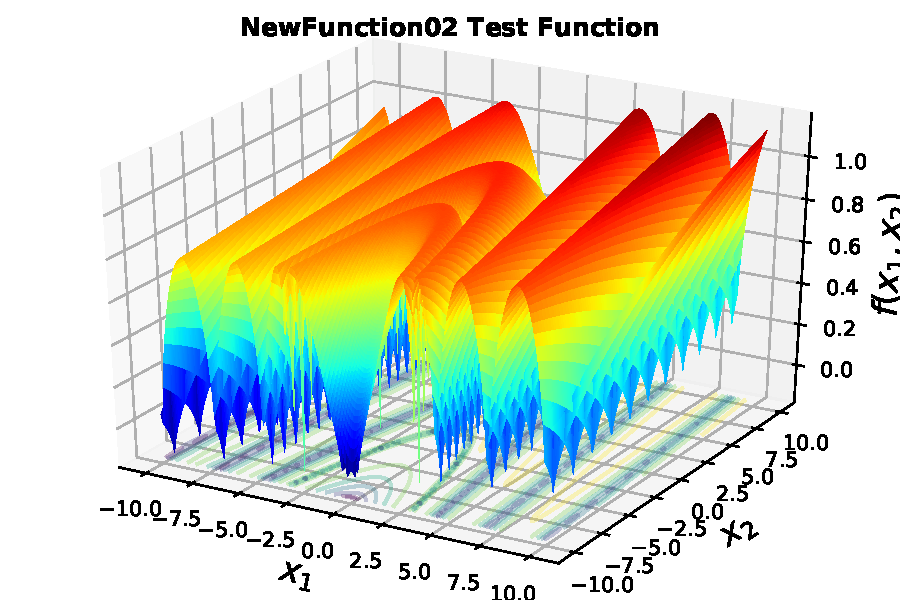
\includegraphics[width=.55\textwidth]{pic/NewFunction02.pdf}
	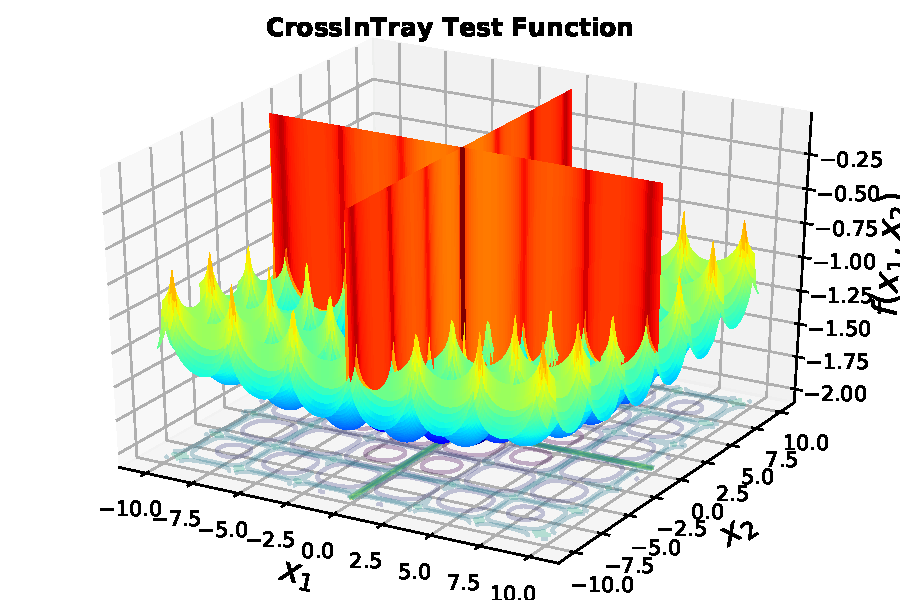
\includegraphics[width=.55\textwidth]{pic/CrossInTray.pdf}%\hfill
\end{figure}
\end{textblock}

\begin{textblock}{7.1}(15.7,1.5)
\hrule\medskip
\Head{Results}
%\begin{comment}
%	\begin{figure}
		
%		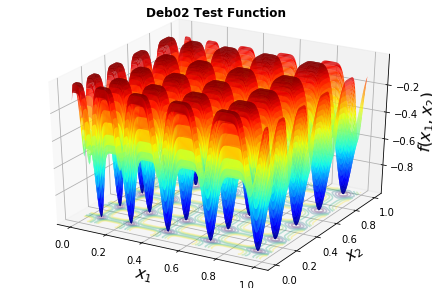
\includegraphics[width=.55\textwidth]{pic/Deb02.png}%\hfill
%		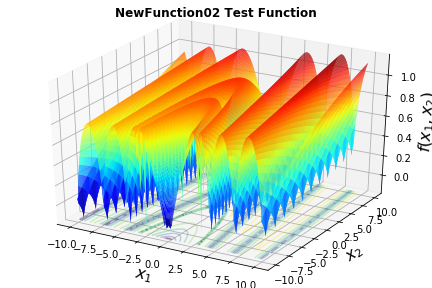
\includegraphics[width=.55\textwidth]{pic/NewFunction02.png}\\
%		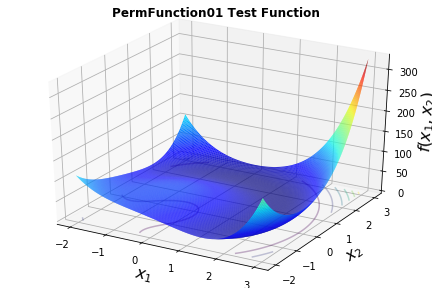
\includegraphics[width=.55\textwidth]{pic/PermFunction01.png}
%		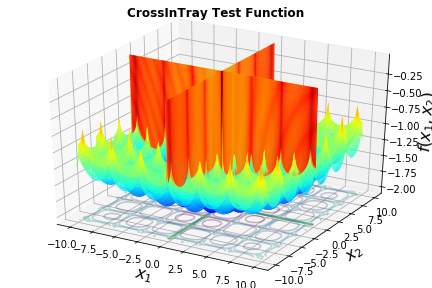
\includegraphics[width=.55\textwidth]{pic/CrossInTray.png}
%	\end{figure}
%\end{comment}
\begin{figure}
	\
	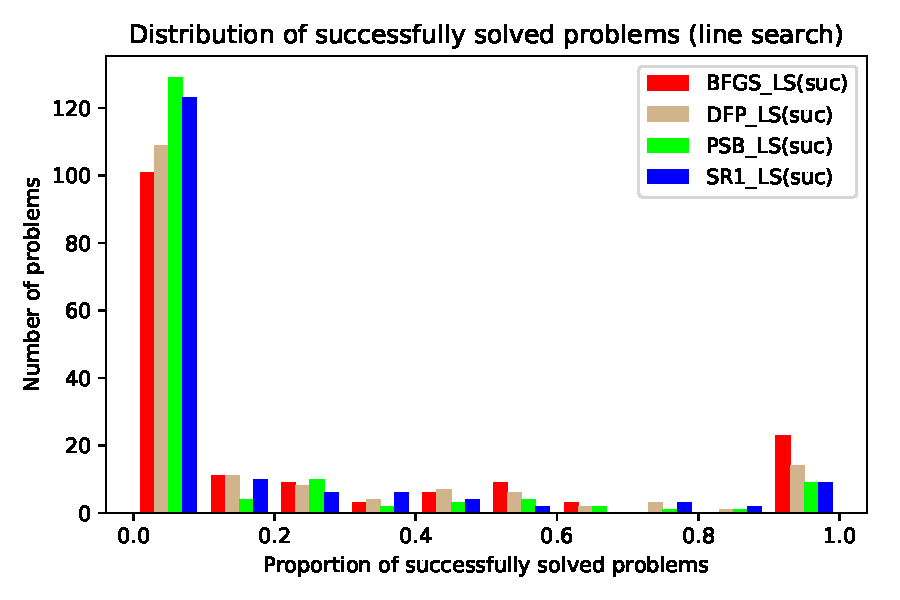
\includegraphics[width=.55\textwidth]{pic/distr_line_search.pdf}
	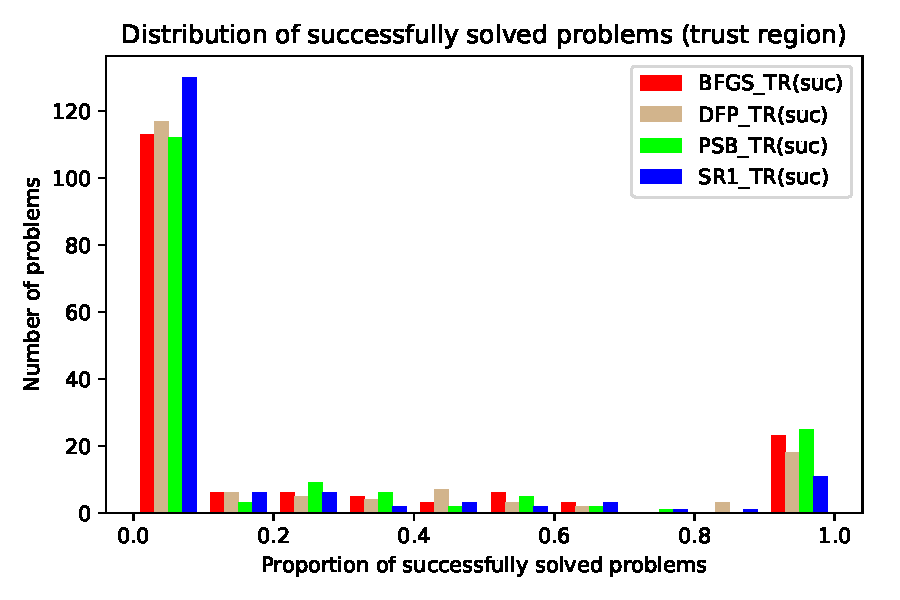
\includegraphics[width=.55\textwidth]{pic/distr_trust_region.pdf}%\hfill
\end{figure}

Proportion of problems that have been successfully solved in more than half and in all launches respectively from random point of domain

%\multicolumn{7}{|c|}{F}

\begin{flushleft}
	\begin{tabular}{ p{5cm} |p{2cm}|p{2cm}|p{2cm}|p{2cm}|p{2cm}|p{2cm}|p{2cm}|p{2cm}|p{2cm}|p{2cm} }
		Strategy	& \multicolumn{2}{c|}{BFGS} & \multicolumn{2}{c|}{DFP} & \multicolumn{2}{c|}{PSB} & \multicolumn{2}{c|}{SR1} & \multicolumn{2}{c}{Total}\\
		\hline
		Line search &0.21 &0.12& 0.16 &0.08&0.09 &0.05&0.09 &0.05&0.07 &0.04\\
		\hline
		Trust region&0.18&0.12&0.16&0.1& 0.19&0.14&0.11&0.06&0.1&0.05
	\end{tabular}
\end{flushleft}

Performance evaluation:
$n_s$ - number of solvers, $n_p$ -  number of problems,
$t_{s,p}$ - time, $r_{s,p} = \fr{t_{s,p}}{\min\{t_{s,p}: s\in S\}}$ - performance profile function\\
$\rho_s(\tau) = \fr{1}{n_p}size\{p:1\le p\le n_p, \quad\log(r_{s,p}\le \tau)\}$ - defines the probability for solver $s$ that the performance ratio $r_{s,p}$ is within a factor $\tau$ of the best possible ratio

\begin{figure}
	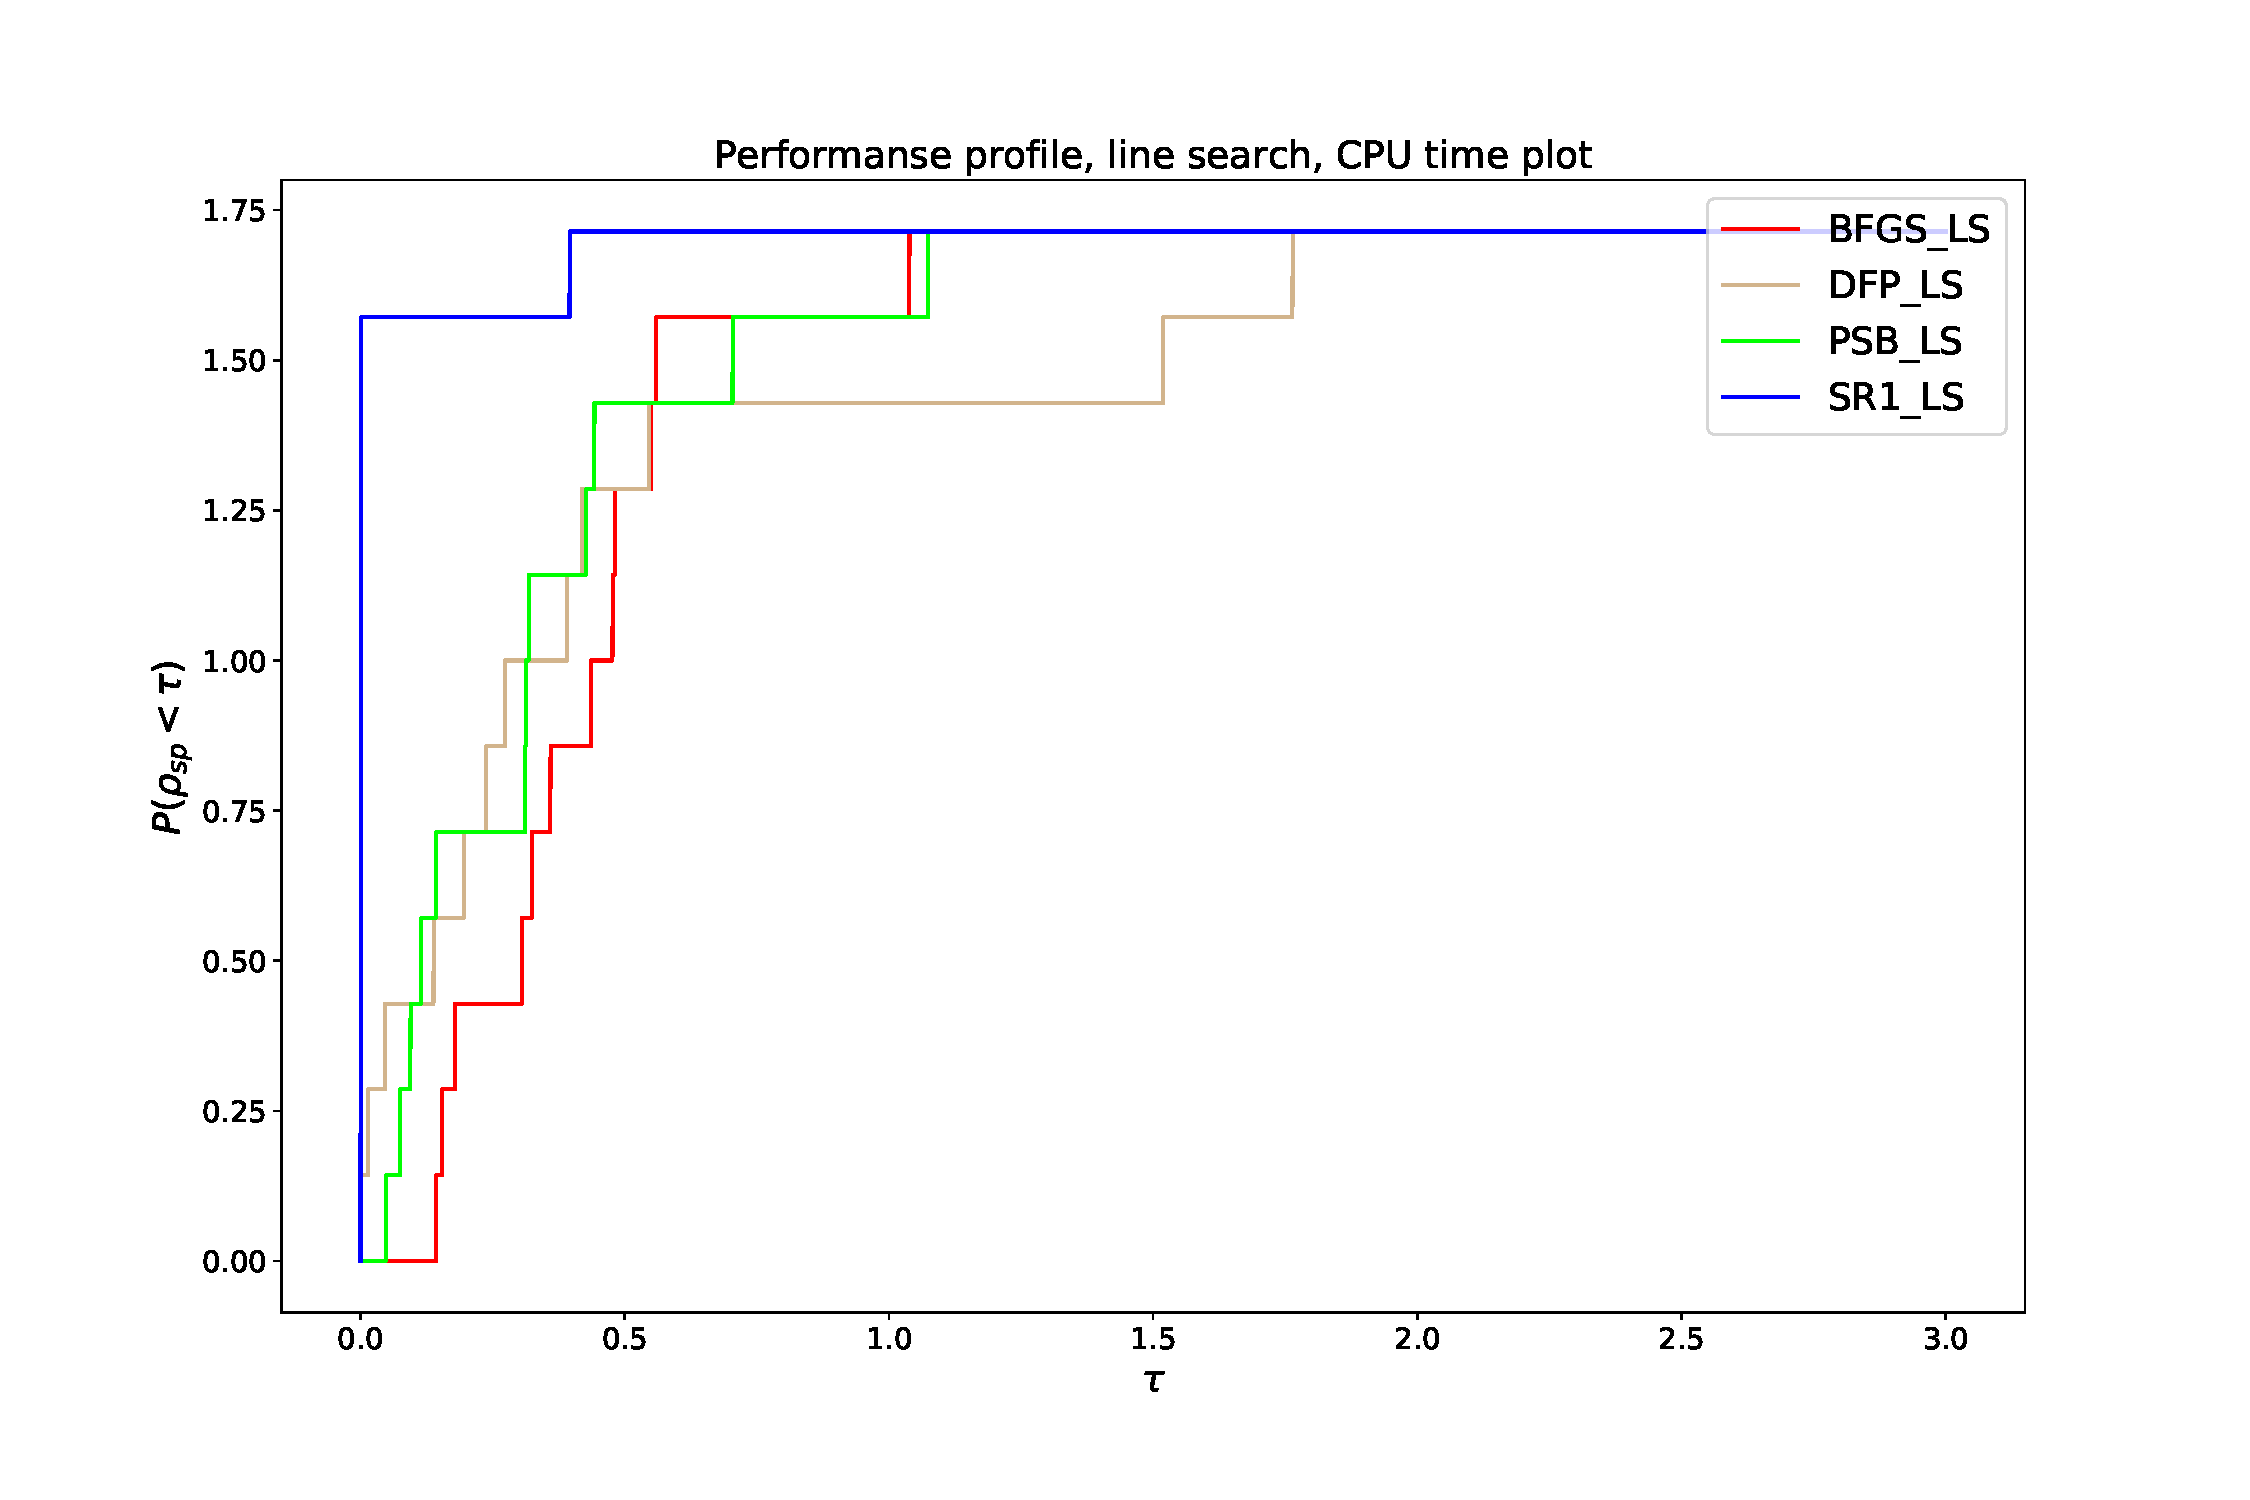
\includegraphics[width=.57\textwidth]{pic/line_search_profiling.pdf}
	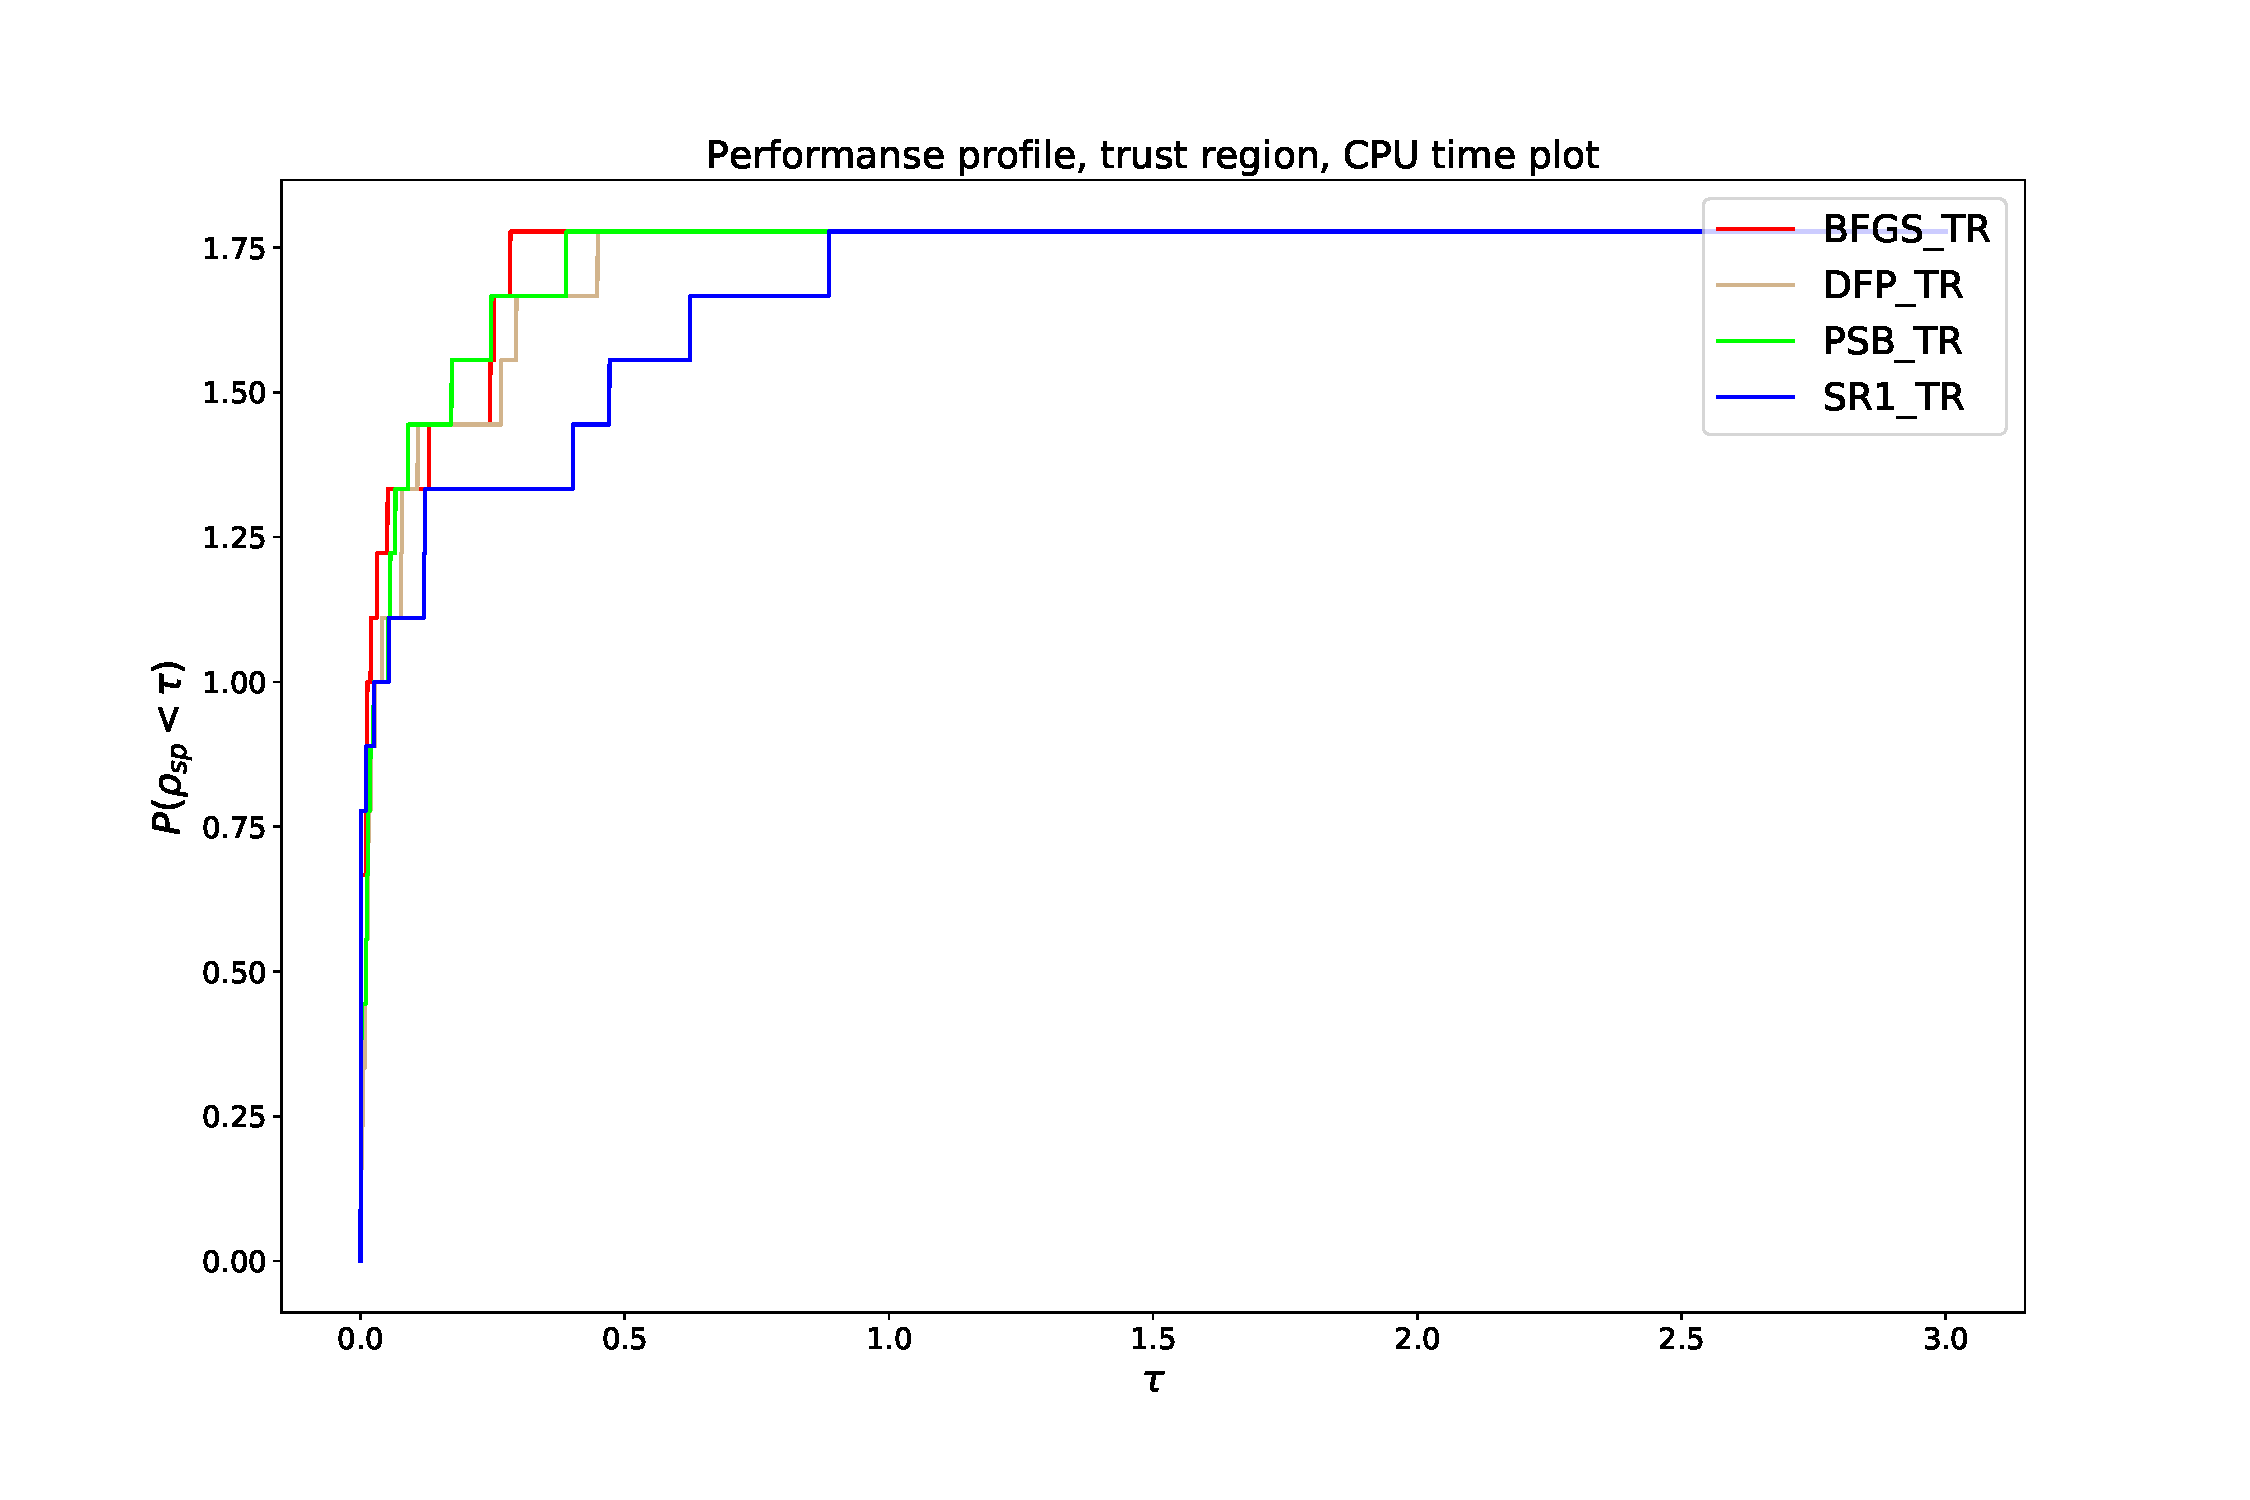
\includegraphics[width=.57\textwidth]{pic/trust_region_profiling.pdf}
\end{figure}

\Head{Conclusions and Further Work}\\
\medskip
\hrule\medskip
\Head{Acknowledgements}\\
The author of the project expresses gratitude to Daniil Merkulov for his lectures of optimization and his support in this project.

\hrule\medskip
\Head{Bibliography}
\begingroup
\renewcommand{\section}[2]{}%
%\renewcommand{\chapter}[2]{}% for other classes
\begin{thebibliography}{}
	\bibitem{Lushi}Ding, Yang, Enkeleida Lushi, and Qingguo Li. "Investigation of quasi-Newton methods for unconstrained optimization." Simon Fraser University, Canada (2004). 
	\bibitem{Nocedal} Wright, Stephen, and Jorge Nocedal. Numerical optimization. Springer Science 35.67-68 (1999)
	\bibitem{Dolan}Dolan, Elizabeth D., and Jorge J. Moré. "Benchmarking optimization software with performance profiles." Mathematical programming 91.2 (2002): 201-213.
\end{thebibliography}
\endgroup

\end{textblock}


\end{document}